\chapter{Care centers characterization}

\section{Motivation}

Countries, such as the UK, USA and Canada, have been implementing a policy of
centralizing the care of patients for many specialized services
\cite{kelly_are_2016}. With such policy, patients are directed to a limited
number of hospitals with higher volumes and more specialized surgeons. There is
evidence that this process will have a positive impact on the health outcomes of
those patients treated in these specialized centres. For instance, centralized
care is beneficial for patients undergoing high-risk procedures, these surgeries
have lower mortality rates when performed by high-volume surgeons
\cite{pekala_centralization_2021,birkmeyer_surgeon_2003,finks_trends_2011,
    hollenbeck_getting_2007,goossens-laan_systematic_2011}. A centralized service
for ovarian cancer may lead to better survival outcomes; evidence from various
other sources suggests that this may also be more cost-effective
\cite{woo_centralisation_2012}. With the rural exodus, the sparsely populated
areas expanded, and several hospitals are serving relatively small populations.
As a result, surgeons operating in these facilities are managing fewer cases of
a given disease. For instance, in the South West of England, surgeons treating
epithelial ovarian cancer were managing fewer than ten cases of ovarian cancer
per year. There is a need to maintain a critical volume of work in order to
sustain surgical expertise \cite{olaitan_surgical_2001}. Finally, a centralized
model of acute stroke care, was found to reduce mortality and length of hospital
stay \cite{morris_impact_2014}.

Through all these evidences, it is clear that not all the hospitals are equal
for cancer treatment. In France, there are many hospitals that do not have
the same degree of oncology specialization. Hospitals are classified into
different legal categories like public hospitals or private structures, but
there is no indicator to assess the degree of oncology specialization and
how large the hospital is. In this chapter, we proposed a method to automatically
label all the hospitals in metropolitan France, based on their statistics and
available health services.

\section{Methods}

\subsection{Labelling hospitals by oncology specialization}

\subsubsection{Data collection}

In this section, we detail how we gathered the data collection process to run
our method.  We first needed health data to characterize the care centers. Then,
geographical and socio-demographic data was used to obtain information on the
population locations. Health data is collected from two sources: the \ac{pmsi}
and the \ac{sae} databases. The \ac{pmsi} database is includes discharge
summaries for all inpatients admitted to public and private hospitals in France.
The \ac{sae} database is a compulsory and exhaustive administrative survey of
all public and private hospitals in France. The survey is sent every year and
describes the activities of the hospitals as well as the list of services and
activities they provide. The list of hospitals in France is available in the
\ac{pmsi} database and updated yearly. There were 5,148 hospitals in 2018. To
obtain statistics on these care centers, we use the \ac{sae} database. There are
more than 50 tables in the \ac{sae}. Only four tables were necessary. We start
with the table ``filtre'' (n=4,041 hospitals) that gathers the general
information about the hospital and the list of services it has. Then we use the
``mco'' table (n=1,650 hospitals) which contains statistics on care centers with
medical surgery or obstetric activity. The table ``cancero'' (997 hospitals)
gathers statistics about oncology activity. Finally, the table ``blocs'' (1,057
hospitals) gathers information about surgery room activity. We merge the care
centers dataset extracted from the \ac{pmsi} with the \ac{sae} tables.
``finess'', ``filtre'' and ``mco'' are merged with an inner join. This operation
will remove care centers that do not declare MCO activity in the \ac{sae}. The
tables ``cancero'' and ``blocs'' are merged with a left join, so that care
center with no oncology or surgery activity could remain in the dataset. The
missing values were filled with 0. The final merged dataset has 1,588 care
centers. Metropolitan France is divided into 13 regions, 96 departments, and
around 35,000 municipalities. The number of municipalities changes each year but
is roughly stable. Statistics on municipalities are publicly available on
various governmental open data platforms. Municipalities and their census
statistics are extracted from the \ac{insee} website. The most up to date data
was released in 2021: population data is from 2017 and 2012, socio-demographic
data is from 2018. Municipalities latitude and longitude coordinates are
retrieved from La Poste open data platform. In the \ac{pmsi} database,
municipalities with small population are merged into ``geographic codes'', an
aggregation of one or more municipalities. The list of the geographic codes and
the municipalities they are linked with are retrieved from the \ac{pmsi}
database. We merge the \ac{insee} dataset with coordinates
extracted from La Poste and the geographic codes correspondence. After merging
these tables, the final dataset comprises 13 regions, 96 departments, 34,877
municipalities and 5,608 geographic codes. \cref{fig:data-sources} summarizes
the data sources we cited previously.

\begin{figure}[h]
    \includegraphics[width=0.9\textwidth]{images/camion/databases.png}
    \centering
    \caption{ \textbf{Data sources used to run the hospital characterization
            step}. We first needed health data to characterize the care centers. Then,
        geographical and socio-demographic data was used to obtain information on the
        population locations. }
    \label{fig:data-sources}
\end{figure}

\subsubsection{Variable selection}

After the previous merge on the \ac{sae} health data, we had more than 200
variables for every care center. We selected a list of 24 variables with the
help of medical experts. The list of variables and their description are listed in
\cref{table:sae-variables}. The variables are either binary when they encode the
presence or absence of a service; or continuous when they encode the number of
stays. % TODO: describe the variables here

Even though the ``cancero'' table gives us the number of stays related to
oncology, we created a new variable to encode the oncology activity of a care
center. Indeed, the number of stays for radiotherapy or chemotherapy is usually
much higher than the number or surgery stays, resulting in an
over-representation of these activities compared to surgery. The ``cancero''
table gives us the number of patients and the number of stays with radiotherapy
and chemotherapy per care center. We subtracted the number of radiotherapy and
chemotherapy stays from the number of oncology stays. We named this variable
``cancero\_nb\_stays\_chirmed''. Then we added to this the number of
chemotherapy and radiotherapy patients, resulting in a new variable that we
refer as ``oncology\_activity''. Finally, log transformation is applied to
continuous data and standard scaling (0 mean and unit variance) on every
variable.

\begin{table}[H]
    \centering
    \resizebox{\textwidth}{!}{%
        \begin{tabular}{|l|l|l|l|}
            \hline
            \textbf{\acs{sae} table} & \textbf{Variable name}      & \textbf{Variable definition}                    & \textbf{Distribution}
            \\ \hline
            filtre                   & chirambu                    & Outpatient surgery activity                     & Binary                \\ \hline
            filtre                   & chimio                      & Chemotherapy activity                           & Binary                \\ \hline
            filtre                   & rth                         & Radiotherapy activity                           & Binary                \\ \hline
            filtre                   & bloc                        & Surgery activity                                & Binary                \\ \hline
            filtre                   & bio                         & Medical biology or anatomopathological activity & Binary                \\ \hline
            filtre                   & rea                         & Intensive care unit                             & Binary                \\ \hline
            filtre                   & medic                       & Medication circuit                              & Binary                \\ \hline
            filtre                   & douleur                     & Chronic pain                                    & Binary                \\ \hline
            filtre                   & palia                       & Palliative care                                 & Binary                \\ \hline
            filtre                   & chircancer                  & Cancer surgery                                  & Binary                \\ \hline
            \acs{mco}                & sejhc\_med                  & Number of inpatient medical stays               & Continuous            \\ \hline
            \acs{mco}                & sejhc\_chi                  & Number of inpatient surgery stays               & Continuous            \\ \hline
            \acs{mco}                & sejhp\_med                  & Number of outpatient medical stays              & Continuous            \\ \hline
            \acs{mco}                & sejhp\_chi                  & Number of outpatient surgery stays              & Continuous            \\ \hline
            \acs{mco}                & lit\_mco                    & Number of \acs{mco} beds                        & Continuous            \\ \hline
            blocs                    & salchir                     & Number of surgery operating rooms               & Continuous            \\ \hline
            blocs                    & salambu                     & Operating rooms dedicated to outpatient surgery & Continuous            \\ \hline
            cancero                  & cancero\_A1                 & Use chemotherapy for cancer treatment           & Binary                \\ \hline
            cancero                  & cancero\_A2                 & Use radiotherapy for cancer treatment           & Binary                \\ \hline
            cancero                  & cancero\_A3                 & Has an oncology dedicated unit                  & Binary                \\ \hline
            cancero                  & cancero\_A11                & Number of patients treated with chemotherapy    & Continuous            \\ \hline
            cancero                  & cancero\_A17                & Number of patients treated with radiotherapy    & Continuous            \\ \hline
            -                        & cancero\_nb\_stays\_chirmed & Number of oncology medical or surgery stays     & Continuous            \\ \hline
            -                        & cancero\_activity           & Oncology activity                               & Continuous            \\ \hline
        \end{tabular}}
    \caption{
        \textbf{List of the variables used for clustering, and their definitions.}
        All the variables except
        cancero\_nb\_stays\_chirmed and cancero\_activity are coming from \ac{sae}.
        The variables are either binary or continuous. Oncology activity is the sum
        of cancero\_nb\_stays\_chirmed, cancero\_17 and cancero\_A11.
    }
    \label{table:sae-variables}
\end{table}

\subsubsection{\acf{pca}}

\ac{pca} is dimensionality-reduction method. It is used to reduce the
dimensionality of large data sets, by transforming a large set of variables into
a smaller one. The new dataset still contains most of the information in the
large set. Dimensionality reduction trades accuracy for simplicity and has
multiple ad- vantages. First, dimensionality reduction removes redundant and
highly correlated features. Then training statistical models on reduced data is
easier and less computationally expensive. Moreover, dimensionality reduction
makes it possible to visualize large dimensional data. In practice, \ac{pca}
projects the original data onto new directions, referred as components. Each
component explains some of the variance from the original dataset. Keeping the
$n$ components with maximum variance and dropping the other ones performs the
actual dimensionality reduction. We call ``explained variance'' the sum of the
variance explained by the components kept. \ac{pca} is relatively easy to
interpret, as each component is a linear combination of the input variables. The
contributions of each input variable to the \ac{pca} components are called
loading scores. We apply the \ac{pca} algorithm to the SAE dataset that
describes the care centers. We used Python's scikit-learn
\cite{pedregosa_scikit-learn_2011} implementation of the \ac{pca}, since it's
very well documented and maintained. The input data has 24 variables, and we
perform a dimensionality reduction with $n=2$ components, explaining 63\% of the
total variance. We tried different number of components, from 2 to 5, but we
found 2 gave good and easy to interpret results.
\subsection{Clustering}

Clustering is the task of grouping data points in such a way that points in the
same group are closer to each other than to those in other groups. It is an
unsupervised Machine Learning algorithm and does not need labelled data to train
on. There are different types of clustering methods and different algorithms.
Hard clustering is when each point belongs to a cluster or not. Soft clustering
is when each point belongs to each cluster to a certain degree. There are many
clustering algorithms, surveyed in \cite{xu_comprehensive_2015}. We want to run
a clustering algorithm on the \ac{pca} reduced dataset to automatically isolate
care centers with similar statistics. We tried several algorithms, and, in our
case, Spectral Clustering \cite{luxburg_tutorial_2007} worked best.

%TODO: reformulate this section
Spectral clustering helps us overcome two major problems in clustering: one
being the shape of the cluster and the other is determining the cluster
centroid. K-means algorithm generally assumes that the clusters are spherical or
round. In spectral, the clusters do not follow a fixed shape or pattern. We now
explain more formally how spectral clustering works. Given a set of data points
$x_1, ..., x_n$ and some notion of similarity $s_{ij} \geq 0$ between all pairs
of data points $x_i$ and $x_j$ , the intuitive goal of clustering is to divide
the data points into several groups such that points in the same group are
similar and points in different groups are dissimilar to each other. A nice way
of representing the data is in form of the similarity graph $G = (V, E)$, where
each vertex $v_i$ in this graph represents a data point $x_i$. Two vertices
$x_i$ and $x_j$ are connected if the similarity $s_{ij}$ between them is
positive or larger than a certain threshold, and the edge is weighted by $s_ij$.
The problem of clustering can be reformulated as such: find a partition of the
graph such that the edges between different groups have very low weights, and
the edges within a group have high weights. The input of the spectral clustering
algorithm are the similarity matrix $S \in \mathbb{R}^{n \times n}$ and the
number of clusters $k$ to construct. From the similarity matrix, we compute the
weighted adjacency matrix $W = (w_{ij})_{i,j=1, ..., n}$, where $w_{ij}$ is the
weight carried by the edge between two vertices $x_i$ and $x_j$. If the two
vertices are not connected, $w_{ij}=0$. The degree $d_i$ of a vertex $v_i \in V$
is defined as the sum of all its related weights $w_{ij}$. The degree matrix $D$
is the diagonal matrix with degrees $d_1, ..., d_n$ on the diagonal. From
the $W$ and $D$ matrices, we compute the unnormalized laplacian $L=D-W$. Then,
we compute the first $k$ eigenvectors $u_1, ..., u_k$ of $L$, and let
$U \in \mathbb{R}^{n \times k}$ be the matrix containing the eigenvectors as
columns. Then, let $y_i \in \mathbb{R}^k$ be the vector corresponding to the
$i$-th row of $U$. Cluster the points $(y_i)_{i=1,...,n}$ with the k-means
algorithm into clusters $C_1, ..., C_k$.

Again, we used Python's scikit-learn Machine Learning library
\cite{pedregosa_scikit-learn_2011}, which implemented the spectral clustering
algorithm. The parameters were left as default. Hence, the affinity matrix was
computed using a radial basis function kernel: $exp(d(X, X)^2)$ with $X$ the
input matrix and $d(X, X)$ the euclidean distance. Regarding the number $k$ of
clusters, we tried various values from 2 to 10 and manually interpreted the
results with medical experts. We found that 8 clusters gave the most
interpretable groups.

\subsection{Grouping hospitals based on their collaborations}

We are now interested in clustering the hospitals based on patients transfers.
We call co-occurrence between two hospitals the number of patients that visited
these two hospitals during its care pathway. The larger the co-occurrence number
is, the more collaboration there is between the two hospitals. We model the
hospitals and their collaborations as a graph, where the nodes are the
hospitals, and the edges are weighted by the number of co-occurrences between
the hospitals. The task we wish to achieve is community detection over this
graph. Intuitively, we seek to find communities of hospitals that frequently
interact together by exchanging patients. Community detection algorithms are
used to evaluate how groups of nodes are clustered or partitioned together.
Detecting communities on graphs is a very active research topic, with many
concrete applications \cite{fortunato_community_2010}. There are different ways
to perform community detection on a graph \cite{hamilton_representation_2018}.
Several approaches have been developed to learn latent node representations
based on the graph topology. These latent representations encode the graph
structure in a continuous vector space, that can be exploited by statistical
models \cite{perozzi_deepwalk_2014}. Learning graph representations was
traditionally performed with Laplacian regularization. However, research shifted
towards learning graph embeddings \cite{kipf_semi-supervised_2017}, inspired by
the skip-gram model \cite{mikolov_distributed_2013}. With such approaches, node
embeddings are learned so that nodes that are strongly connected are close in
the latent space. Once the embeddings are learned, common statistical learning
tasks can be performed such as graph classification, link prediction, or
community detection \cite{hamilton_representation_2018}. Recently, \ac{vgae} were introduced to learn latent representations for
undirected graphs, in an unsupervised manner \cite{kipf_variational_2016}. This
framework is based on the Variational Auto Encoder model
\cite{kingma_auto-encoding_2014}, with a \ac{gcn}
\cite{kipf_semi-supervised_2017} encoder and an inner-product decoder. \ac{gcn}
are similar to regular Convolution Layers used mostly in computer vision. In
computer vision, the input neurons are multiplied with a set of weights that are
commonly known as filters or kernels. The filters act as a sliding window across
the whole image and enable to learn higher level features from the neighboring
cells. In \ac{gcn}, the filters are moved across the graph nodes, and learn
features from the neighboring nodes. The hidden representation of a given
node can be obtained as the average value of the current node features along
with its neighbors. Based on the learned representations of every node,
the inner-product decoder aims at reconstructing the adjacency matrix of the
input graph. That way, the network will learn similar latent vectors for nodes
that are strongly connected in the graph. One advantage of this method is that
we can use node features to learn the representations.

In our case, we use the co-occurrence network between the $n$ hospitals as input
graph. This is a non directed weighted graph, where strongly connected nodes are
hospitals with many co-occurrences. We ran the \ac{vgae} model over the
adjacency matrix of the graph, without using nodes features. We a chose a latent
representation  of size $k=32$. The output was a matrix
$Z \in \mathbb{R}^{n \times k }$ corresponding to the embedding vectors
of each hospital node. We ran a TSNE \cite{van_der_maaten_viualizing_2008}
dimensionality reduction algorithm on top of $Z$ to obtain a 2D
representation of every hospital. Finally, we performed a clustering on top of
the reduced data, with the DBSCAN algorithm \cite{ester_density-based_1996}.

\section{Results}

We first describe the spatial distribution and specificities of the 1,662
hospitals included in this study. There are different types of hospitals in
France: \ac{ch}  (n=667) and \ac{chru}  (n=142) are state-run hospitals;
\ac{clcc} (n=26) and \ac{psph} or \ac{ebnl} (n=142) are both private hospitals of
collective interest, though \ac{clcc} are oncology dedicated; private hospitals
(n=606) are privately run and for-profit. The non \ac{mco} care centers with
radiotherapy activity (n=79) are mostly private practice structures and are
referred as “Other”. \cref{table:oncology-activity-per-region} shows the number
of care centers and their oncology activity per hospital type and region. Most
of the care centers are public, but a non-insignificant part are private.
\ac{clcc} represent only 1.6\% of the care centers, yet they are responsible for
14.2\% of the overall oncology activity. The care centers are unevenly
distributed across the country. For instance, Corse and Centre-Val-de-Loire are
the only two regions with no \ac{clcc} care centers. Moreover, the proportion of
oncology activity per hospital type varies from a region to another. For
instance, in Nouvelle-Aquitaine, 47.1\% of the oncology activity is handled by
private care centers, whereas in Provence-Alpes-Cote-d'Azur it is 21.4\%.

\begin{table}[H]
    \resizebox{\textwidth}{!}{%
        \begin{tabular}{|l|l|l|l|l|l|l|l|l|}
            \hline
            \textbf{Variable value per region}                & ~               & \multicolumn{7}{c|}{\textbf{Hospital Type}}                                                                            \\
            \hline
            N = number of centers                             & ~               & \acs{ch}                                    & \acs{ch}        & \acs{clcc}       & Other          &
            \acs{psph}/\acs{ebnl}                             & Privé           & All                                                                                                                    \\
            A = oncology activity (radio. + chemo. + surgery) & ~               & (n=667)                                     &
            (n=142)                                           & (n=26)          & (n=79)                                      & (n=142)         & (n=606)          & n=1,662                             \\ \hline
            Auvergne-Rhône-Alpes                              & N               & 98 (49,2\%)                                 & 21 (10,6\%)     & 2 (1\%)          & 7
            (3,5\%)                                           & 13 (6,5\%)      & 58 (29,1\%)                                 & 199                                                                      \\
            ~                                                 & A               & 34,597 (26,7\%)                             & 31,706 (24,5\%) & 16,966 (13,1\%)  & 6,710
            (5,2\%)                                           & 6,146 (4,7\%)   & 33,297 (25,7\%)                             & 129.422                                                                  \\ \hline
            Bourgogne-Franche-Comté                           & N               & 53 (64,6\%)                                 & 4 (4,9\%)       & 1 (1,2\%)        & 5
            (6,1\%)                                           & 2 (2,4\%)       & 17 (20,7\%)                                 & 82                                                                       \\
            ~                                                 & A               & 12,238 (27,6\%)                             & 10,621 (24\%)   & 5,844 (13,2\%)   & 4,405 (9,9\%)
                                                              & 657 (1,5\%)     & 10,571 (23,8\%)                             & 44.336                                                                   \\ \hline
            Bretagne                                          & N               & 38 (33\%)                                   & 8 (7\%)         & 1 (0,9\%)        & 6 (5,2\%)      & 11 (9,6\%)
                                                              & 51 (44,3\%)     & 115                                                                                                                    \\
            ~                                                 & A               & 15,953 (27\%)                               & 11,020 (18,6\%) & 6,341 (10,7\%)   & 5,553 (9,4\%)
                                                              & 2,050 (3,5\%)   & 18,199 (30,8\%)                             & 59.116                                                                   \\ \hline
            Centre-Val de Loire                               & N               & 29 (46,8\%)                                 & 4 (6,5\%)       & 0 (0\%)          & 6 (9,7\%)
                                                              & 2 (3,2\%)       & 21 (33,9\%)                                 & 62                                                                       \\
            ~                                                 & A               & 6,989 (19,6\%)                              & 11,524 (32,2\%) & 0 (0\%)          & 5,137 (14,4\%) & 32
            (0,1\%)                                           & 12,058 (33,7\%) & 35.74                                                                                                                  \\ \hline
            Corse                                             & N               & 7 (53,8\%)                                  & 0 (0\%)         & 0 (0\%)          & 0 (0\%)        & 0 (0\%)    & 6
            (46,2\%)                                          & 13                                                                                                                                       \\
            ~                                                 & A               & 3,486 (66,3\%)                              & 0 (0\%)         & 0 (0\%)          & 0 (0\%)        & 0 (0\%)    & 1,773
            (33,7\%)                                          & 5.259                                                                                                                                    \\ \hline
            Grand Est                                         & N               & 70 (41,7\%)                                 & 17 (10,1\%)     & 3 (1,8\%)        & 6 (3,6\%)      & 30
            (17,9\%)                                          & 42 (25\%)       & 168                                                                                                                    \\
            ~                                                 & A               & 17,428 (19,6\%)                             & 22,123 (24,9\%) & 13,176 (14,8\%)  & 6,793
            (7,7\%)                                           & 7,683 (8,7\%)   & 21,553 (24,3\%)                             & 88.756                                                                   \\ \hline
            Hauts-de-France                                   & N               & 56 (40\%)                                   & 11 (7,9\%)      & 1 (0,7\%)        & 11 (7,9\%)     &
            12 (8,6\%)                                        & 49 (35\%)       & 140                                                                                                                    \\
            ~                                                 & A               & 21,864 (26\%)                               & 15,934 (19\%)   & 6,947 (8,3\%)    & 8,618 (10,3\%) &
            5,242 (6,2\%)                                     & 25,399 (30,2\%) & 84.004                                                                                                                 \\ \hline
            Île-de-France                                     & N               & 40 (47,6\%)                                 & 5 (6\%)         & 4 (4,8\%)        & 6 (7,1\%)      & 3
            (3,6\%)                                           & 26 (31\%)       & 84                                                                                                                     \\
            ~                                                 & A               & 7,573 (14,9\%)                              & 7,947 (15,7\%)  & 14,210 (28\%)    & 5,419 (10,7\%)
                                                              & 0 (0\%)         & 15,627 (30,8\%)                             & 50.776                                                                   \\ \hline
            Normandie                                         & N               & 70 (44,9\%)                                 & 10 (6,4\%)      & 1 (0,6\%)        & 7 (4,5\%)      & 12
            (7,7\%)                                           & 56 (35,9\%)     & 156                                                                                                                    \\
            ~                                                 & A               & 37,844 (33\%)                               & 26,244 (22,9\%) & 7,477 (6,5\%)    & 7,157 (6,2\%)
                                                              & 2,824 (2,5\%)   & 33,271 (29\%)                               & 114.817                                                                  \\ \hline
            Nouvelle-Aquitaine                                & N               & 66 (37,7\%)                                 & 14 (8\%)        & 2 (1,1\%)        & 7 (4\%)        &
            6 (3,4\%)                                         & 80 (45,7\%)     & 175                                                                                                                    \\
            ~                                                 & A               & 14,735 (12,1\%)                             & 20,915 (17,2\%) & 16,047 (13,2\%)  & 11,572
            (9,5\%)                                           & 1,098 (0,9\%)   & 57,374 (47,1\%)                             & 121.741                                                                  \\ \hline
            Occitanie                                         & N               & 34 (44,7\%)                                 & 5 (6,6\%)       & 3 (3,9\%)        & 4 (5,3\%)      & 5
            (6,6\%)                                           & 25 (32,9\%)     & 76                                                                                                                     \\
            ~                                                 & A               & 11,901 (18,9\%)                             & 11,374 (18,1\%) & 12,564 (19,9\%)  & 3,422
            (5,4\%)                                           & 3,916 (6,2\%)   & 19,822 (31,5\%)                             & 62.999                                                                   \\ \hline
            Pays de la Loire                                  & N               & 53 (34,4\%)                                 & 10 (6,5\%)      & 3 (1,9\%)        & 4 (2,6\%)
                                                              & 15 (9,7\%)      & 69 (44,8\%)                                 & 154                                                                      \\
            ~                                                 & A               & 14,632 (13,6\%)                             & 16,533 (15,4\%) & 21,924 (20,4\%)  & 6,172
            (5,7\%)                                           & 10,918 (10,2\%) & 37,176 (34,6\%)                             & 107.355                                                                  \\ \hline
            Provence-Alpes-Côte d'Azur                        & N               & 53 (22,3\%)                                 & 33 (13,9\%)     & 5 (2,1\%)        &
            10 (4,2\%)                                        & 31 (13\%)       & 106 (44,5\%)                                & 238                                                                      \\
            ~                                                 & A               & 24,390 (12,6\%)                             & 66,406 (34,2\%) & 34,028 (17,5\%)  & 12,817
            (6,6\%)                                           & 14,981 (7,7\%)  & 41,577 (21,4\%)                             & 194.199                                                                  \\ \hline
            Grand Total                                       & N               & 667 (40,1\%)                                & 142 (8,5\%)     & 26 (1,6\%)       & 79 (4,8\%)     &
            142 (8,5\%)                                       & 606 (36,5\%)    & 1662                                                                                                                   \\
            ~                                                 & A               & 223,630 (20,4\%)                            & 252,347 (23\%)  & 155,524 (14,2\%) & 83,775
            (7,6\%)                                           & 55,547 (5,1\%)  & 32,7697 (29,8\%)                            & 1,098,520                                                                \\ \hline
        \end{tabular}} \caption{ \textbf{Number of care centers (N) and overall
            oncology activity (A) per hospital type and region.} Oncology activity is
        the sum of the number of patients with radiotherapy or chemotherapy, and the
        number of medical or surgery stays related to cancer. \ac{ch} and \ac{chru}
        are public hospitals; \ac{clcc} and \ac{psph}/\ac{ebnl} are private
        hospitals of collective interest, though \acs{clcc} are oncology dedicated;
        private hospitals are for-profit. “Other” hospitals are mostly private
        practice radiotherapy structures. The percentages sum to 100\% row-wise. In
        Nouvelle-Aquitaine, 47.1\% of the oncology activity is handled by private
        care centers, whereas in Provence-Alpes-Cote-d'Azur it is 21.4\%. }
    \label{table:oncology-activity-per-region}
\end{table}

\subsubsection{Oncology specialization label}

While it is obvious that \ac{clcc} care centers are suited for oncology care, it
is difficult to assess the degree of oncology specialization for other care
centers. Our clustering algorithm assigned the n=1,662 care centers into 8
clusters, sorted by oncology specialization. The \ac{pca} and clustering results
are visible on \cref{fig:clustering-pca}. The scatter plots (A) and (B) display
the hospitals as points in the 2-dimensional PCA space, colored by assigned
cluster (A) and hospital category (B). We see two main groups of points on this
scatter plot, one on top and one on the bottom. These points are well separated
along the second PCA component. From plot (C), we can interpret the PCA
components. The first one is correlated with almost every input variable,
meaning that the higher this component is, the larger and the more developed the
hospital is. Regarding the second component, it is correlated with oncology
dedicated variables, especially radiotherapy. This means that hospitals with a
large value along the second component are dedicated to oncology and have a
radiotherapy activity. From this, we understand that points with large values
along the two components are large hospitals with an important oncology
activity. This seems to be the case for hospitals in clusters 1 and 2 (A).
When we look at the hospitals categories on plot (B), we notice that these
points on the top right side of the figure are essentially \ac{clcc}, which
makes sense since these hospitals are fully dedicated to oncology by design.
However, there are also hospitals from all the other categories, which would
have been less easy to identify as oncology experts.

\begin{figure}[H]
    \includegraphics[width=0.9\textwidth]{images/camion/supplemental/sup_fig1_pca_and_clustering.png}
    \centering
    \caption{ \textbf{\ac{pca} interpretation}. Care centers are showed as
        points in the 2-dimensional \ac{pca} space. Points are colored by
        cluster index (A) and hospital type (B). \ac{clcc} care centers are
        close together in the \ac{pca} space, proving they have similar activity
        and services distribution. \ac{pca} components are a linear combination
        of the input variables (C). The loading scores reflect how much the
        input variable contributed to the \ac{pca} component. Component 1 is
        associated with most of the variables, while component 2 is linked with
        radiotherapy variables. Hence, we interpret component 1 as hospital size
        and component 2 as oncology specialization. }
    \label{fig:clustering-pca}
\end{figure}

The \cref{fig:clustering-spider} shows the distribution of some of the key
health services per cluster. These services are biology, radiotherapy,
chemotherapy, cancer surgery, intensive unit, palliative care, oncology unit,
medication circuit, surgery, and outpatient surgery. The three oncology services
are cancer surgery, radiotherapy, and chemotherapy. We see that care centers
from clusters 1 (n=79) and 2 (n=39) all have these 3 services, hence they are
the most suited hospitals for oncology care. Centers from cluster 3 (n=451) have
cancer surgery and chemotherapy but lack radiotherapy. The most part of the
n=381 centers from cluster 4 have cancer surgery, but no radiotherapy nor
chemotherapy. Care centers from cluster 5 (n=2) and cluster 6 (n=7) have
radiotherapy and chemotherapy services, but no cancer surgery. Care centers in
cluster 7 (n=77) are dedicated to radiotherapy and mostly private practice
structures. Finally, care centers 8 (n=626) have none of the 3 oncology
services. To sum up, hospitals from clusters 1 and 2 (n=118) are “all-in-one”
care centers that provide the most “ideal” oncology care. Centers from clusters
3 and 4 (n=382) provide oncology care but will have to be coordinated with
additional structures during the pathways. Hospitals within clusters 5, 6 and 7
(n=86) are not allowed to perform cancer surgery but provide chemotherapy or
radiotherapy. The remaining n=626 care centers in cluster 8 are not equipped for
oncology care.

\begin{figure}[H]
    \includegraphics[width=0.9\textwidth]{images/camion/fig1_clusters_services.png}
    \centering
    \caption{ \textbf{Distribution of the care centers services and equipment
            per cluster.} Each radar plot axis shows the percentage of the care
        centers within the cluster that have the corresponding attribute. In
        Cluster 1, the care centers have all the listed services. In cluster 8,
        the centers have almost none of the services. Care centers from cluster
        1 (n=79) and cluster 2 (n=39) are the most suited for oncology care. }
    \label{fig:clustering-spider}
\end{figure}

We now look at the hospital categories distribution among each cluster. Hospital
types are unevenly distributed among the clusters as illustrated on
\cref{fig:clustering-categories}. For instance, 76.9\% of the \ac{clcc} care
centers are placed in cluster 1, as they are the most specialized centers. In
cluster 7, we find external radiotherapy units of some \ac{clcc} centers, and
private practice structures, classified as ``Other''. The proportion of private
care centers varies as well: cluster 1 has almost no private care center while
cluster 2 has 61.5\% of private hospitals. Thus, it appears that many privately
held hospitals do not have a biology activity, but they have all the other
services. This illustrates that the hospital category could not be used to
assess the oncology specialization, apart from the \ac{clcc} category.

\begin{figure}[h]
    \includegraphics[width=0.9\textwidth]{images/camion/supplemental/sup_fig2_categories_per_cluster.png}
    \centering
    \caption{ \textbf{Comparison between hospital types and assigned clusters.}
        The majority of the \ac{clcc} care centers are grouped together in
        cluster 1. Moreover, cluster 1 has a very low percentage of private
        hospitals, whereas this proportion is the much higher in cluster 2.
        ``Other'' care centers are mostly private practice radiotherapy
        structures, and they are regrouped in cluster 7. }
    \label{fig:clustering-categories}
\end{figure}

The \cref{fig:clustering-cumulative} shows the percentage of oncology activity
covered by each cluster. Most of the oncology activity is handled by care
centers from clusters 1 and 3. The activity of the 79 hospitals
in the cluster 1 combined equals 36.8\% of the total activity.
This is almost as large as the activity of the n=451 hospitals
from cluster 3. As mentioned in the centralization of care benefits, the care
centers from the cluster 1 probably have the largest expertise due to the
large volume of cancer patients they treat.

\begin{figure}[H]
    \includegraphics[width=0.5\textwidth]{images/camion/supplemental/sup_fig3_nb_stays_per_cluster.png}
    \centering
    \caption{ \textbf{Cumulative sum of the oncology activity, per cluster.}
        Most of the oncology activity is handled by care centers from clusters 1
        and 3. While there are only n=79 care centers in cluster 1, their total
        activity is almost as large as the n=451 care centers from cluster 3. }
    \label{fig:clustering-cumulative}
\end{figure}

Finally, we study the spatial distribution of the hospitals in metropolitan
France, and compare it with the population density distribution. In 2018, the
population in France was 66,993 million. Mainland France hosts 64,812 million
inhabitants (96.8\%), while the remaining 2,181 million (3.2\%) live in overseas
departments and regions . Metropolitan France is divided into 13 administrative
regions and 96 departments. The population density in France is unevenly
distributed . In 2020, the overall population density in metropolitan France was
119 inhabitants per square kilometer. Ile-de-France region has the highest
population density with 1,022 inhabitants per square kilometer. Density in other
regions in metropolitan France range between 40 and 187
inhabitants/km\textsuperscript{2}. Denser areas are located near the coastline
and around the largest cities like Paris, Marseille, Lyon, Strasbourg, Toulouse,
or Bordeaux. The middle of the country is rural, and the population densities
are low. While there are a great variety of regions and landscapes, the country
is becoming more urbanized. This ``rural exodus'' is largely responsible of what
is known as the ``empty diagonal'', a band of very low-density population that
stretches from the southwest to the northeast. On \cref{fig:clustering-map}, Map
(A) shows the metropolitan France map, with municipalities colored by population
density cuts. The various bins are: <30; 30-50; 50-100; 100-200; and >200
inhabitants per km\textsuperscript{2}. The hospitals are displayed as
pictograms, sized by oncology activity and colored by their assigned cluster.
Unsurprisingly, the largest hospitals and the most specialized in oncology are
located in densely populated areas. The box plot (B) shows the population
distribution of the municipalities where the hospitals are located, by cluster
index. As expected, the municipalities where hospitals from the cluster 1 are
more populated. Bar plots (C) and (D) show the number of hospitals by cluster
index for every region. Plot (C) shows the absolute number where plot (D) shows
the number of hospitals per 100,000 inhabitants.

\begin{figure}[H]
    \includegraphics[width=0.9\textwidth]{images/camion/supplemental/sup_fig4_care_centers_pop_density.png}
    \centering
    \caption{ \textbf{Care centers spatial distribution, compared with
            population density.} Population density in metropolitan France is
        unevenly distributed across the country (A). Areas in the middle, near
        the Pyrenees and the Alps have very low population densities. The most
        specialized care centers are in dense areas and in large municipalities
        (B). While Ile-de-France has the highest number of care centers, it has
        the least care centers per 100,000 inhabitants. }
    \label{fig:clustering-map}
\end{figure}

\subsubsection{Collaborations between hospitals}

\begin{figure}[H]
    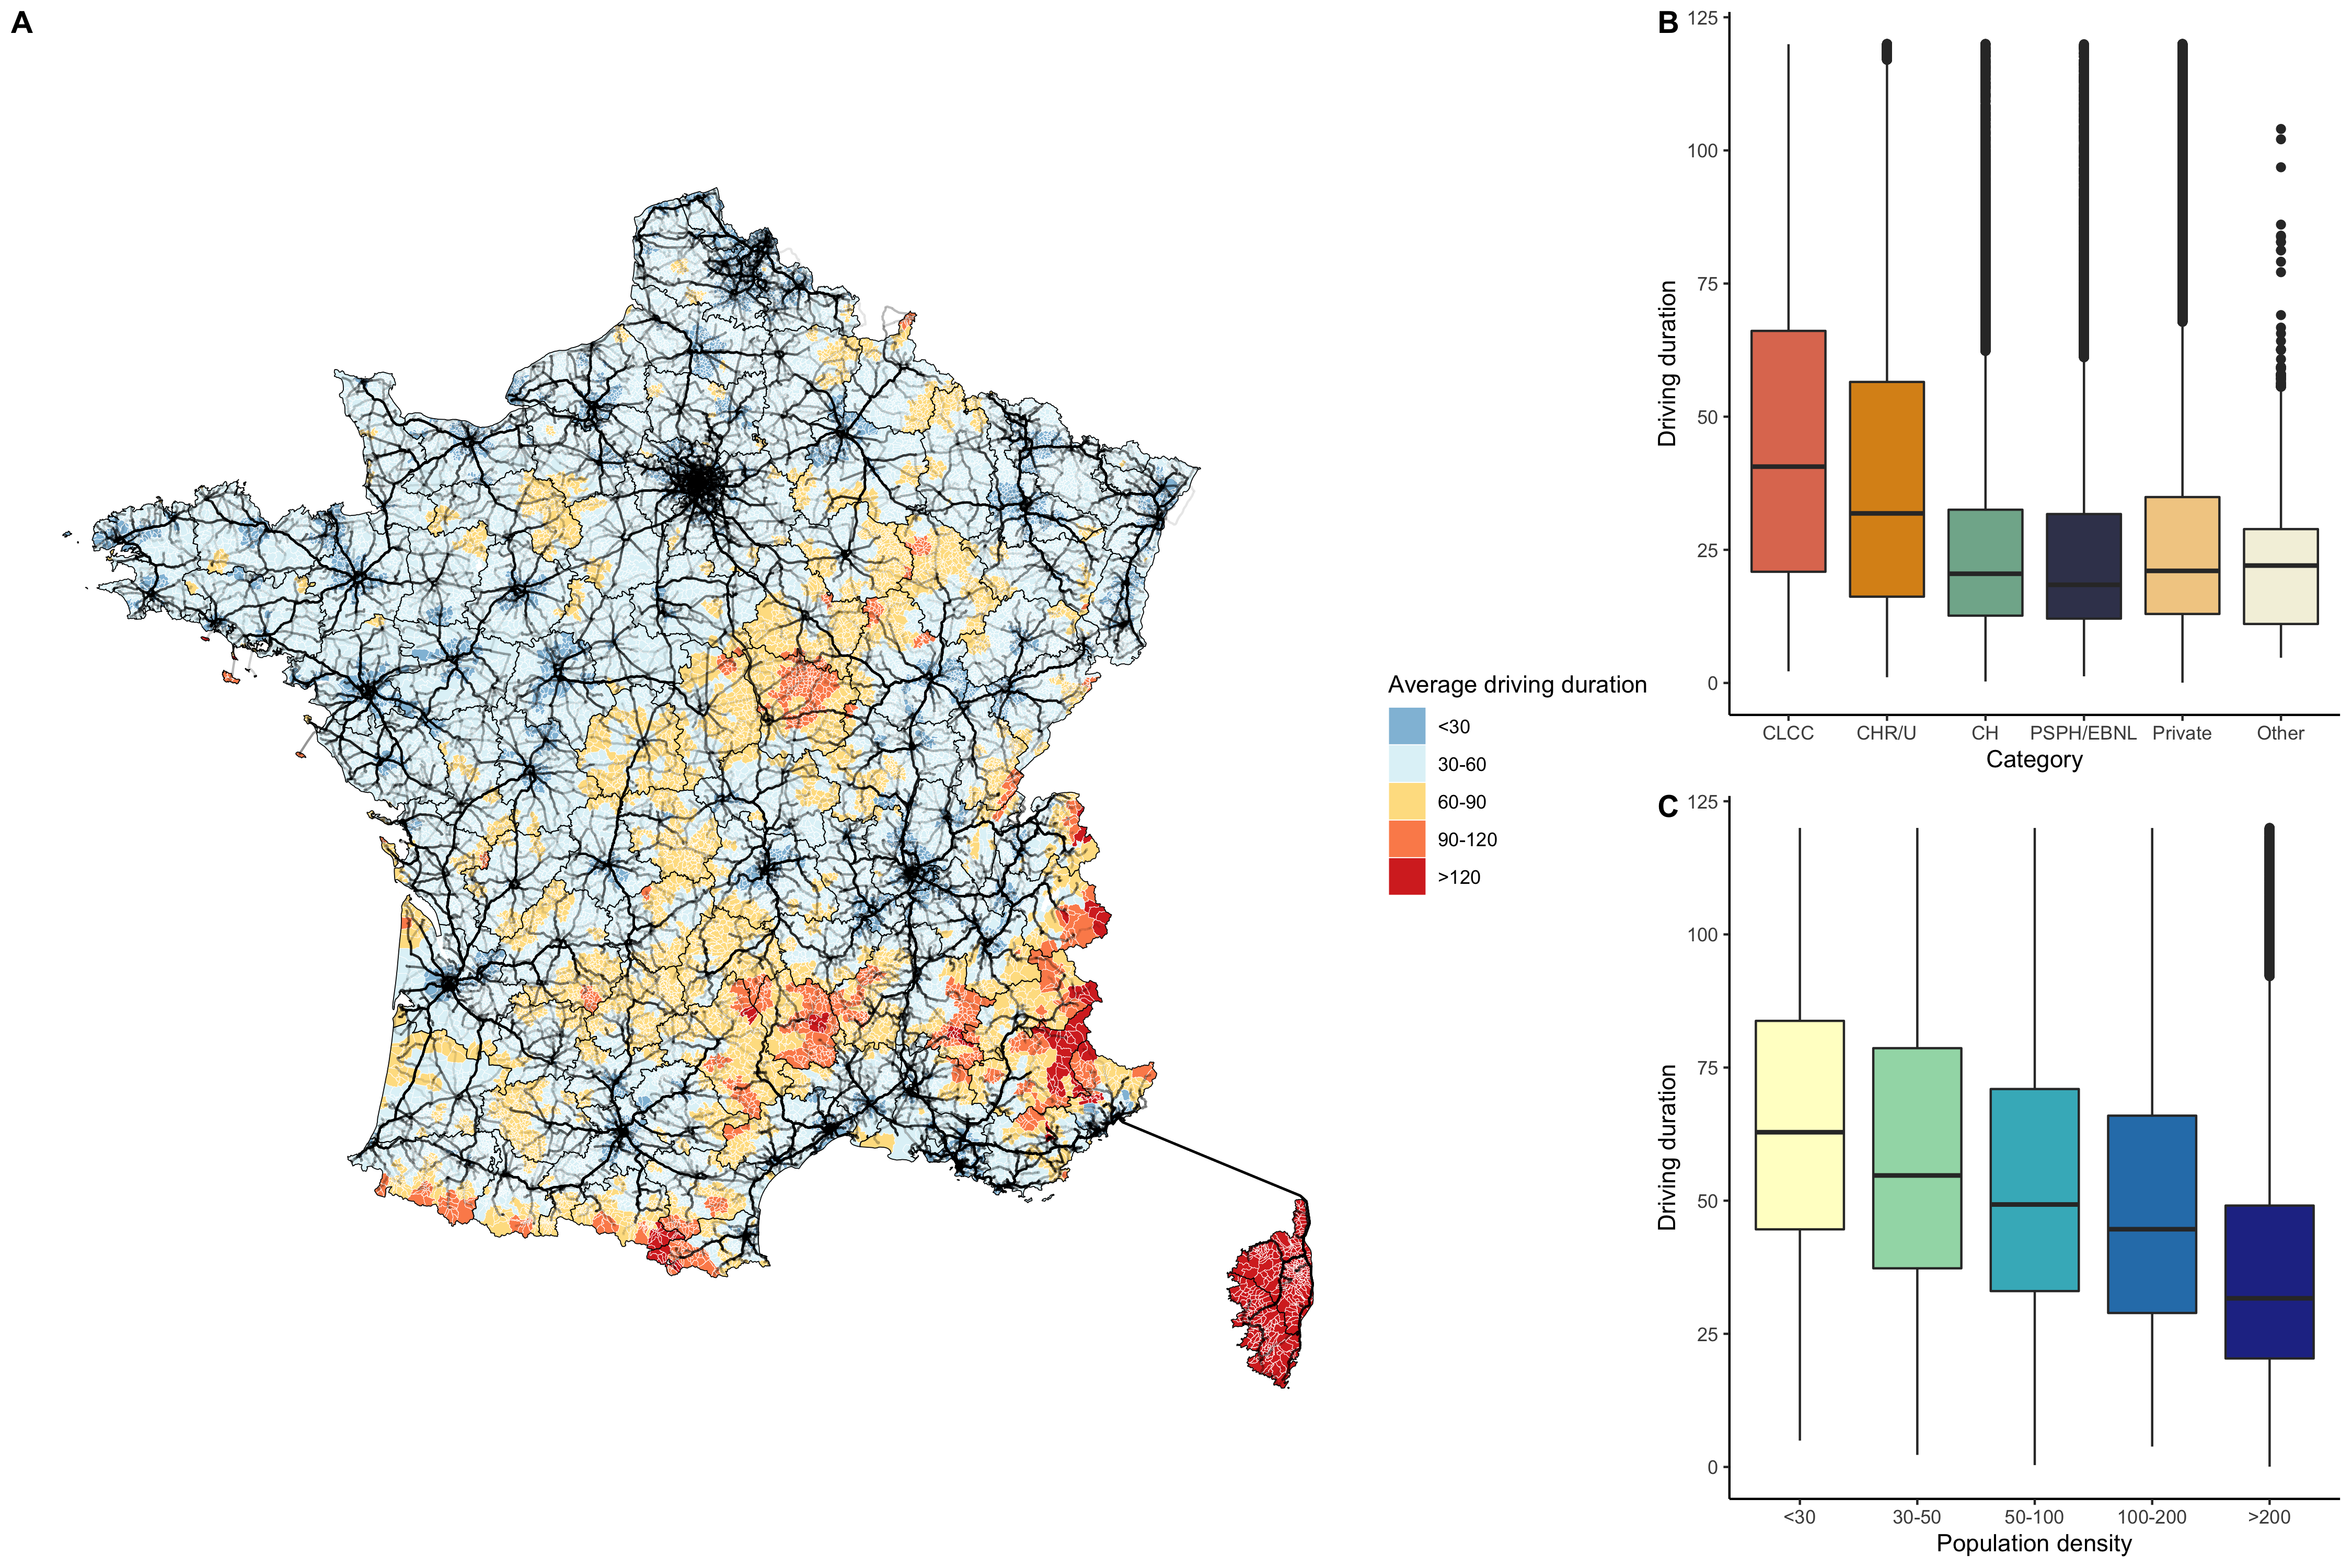
\includegraphics[width=0.9\textwidth]{images/co-occurrences/fig1.png}
    \centering
    \caption{ \textbf{Community detection in France.} Foo }
    \label{fig:co-occ-france}
\end{figure}

\begin{figure}[H]
    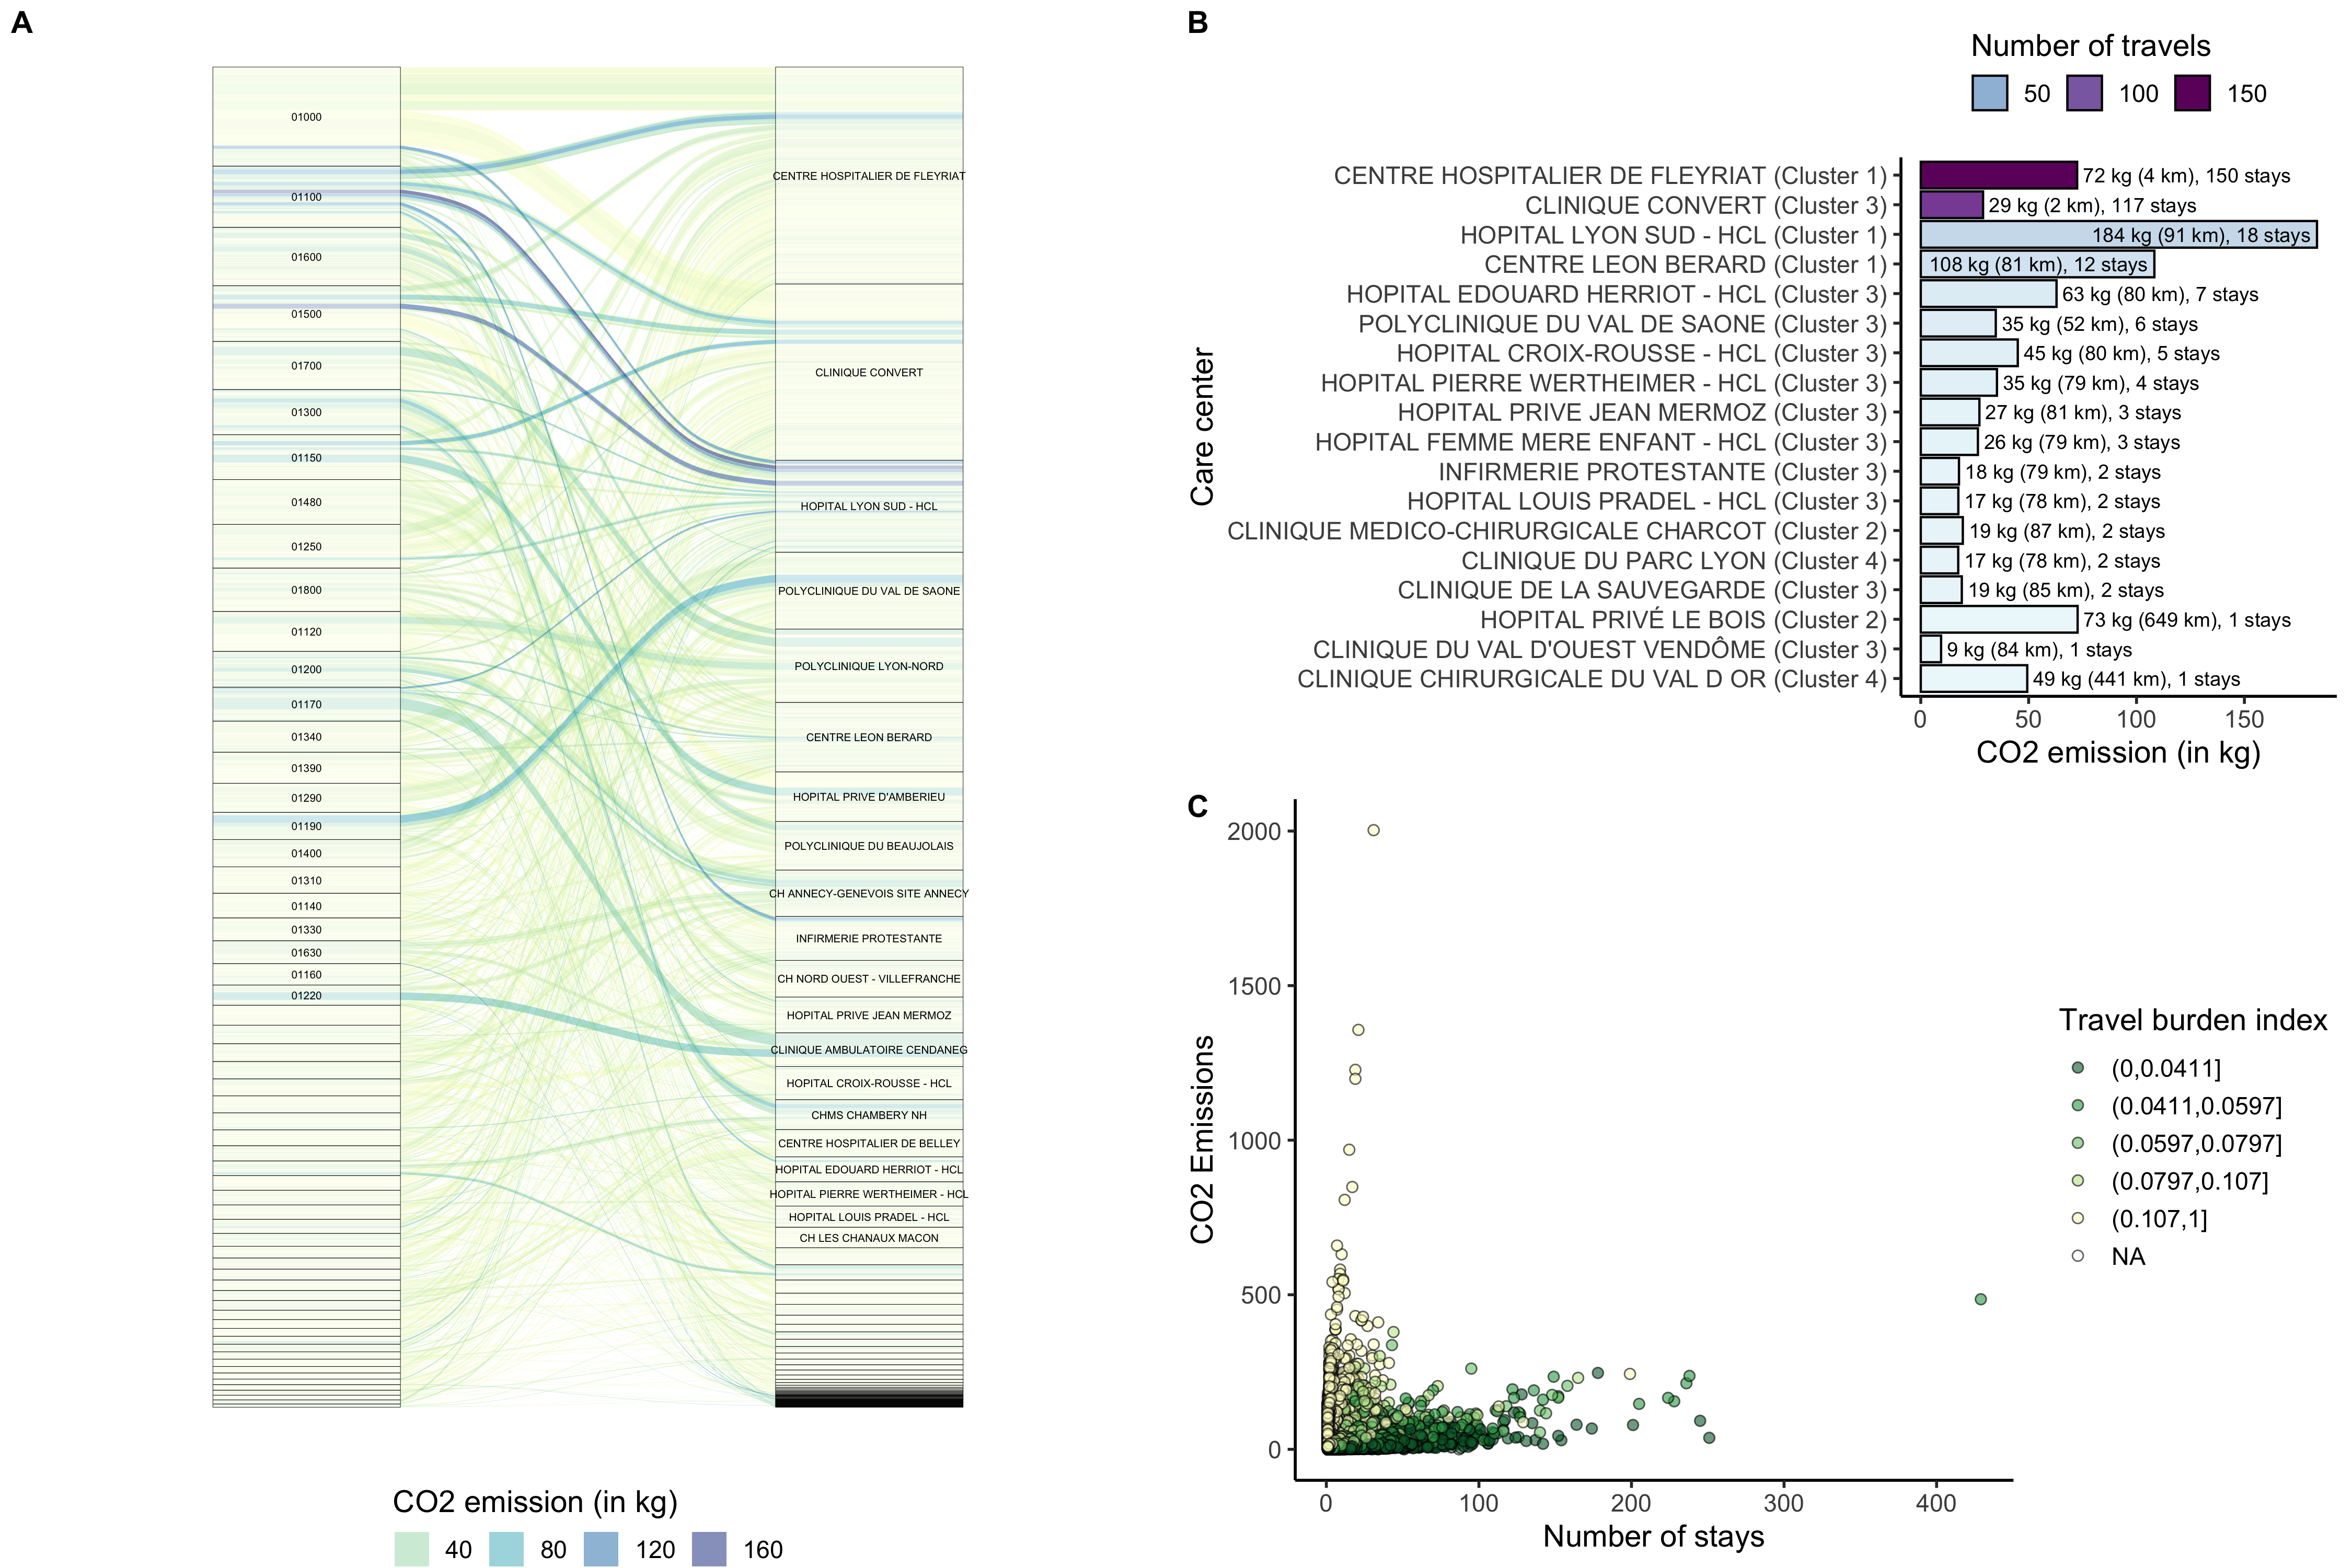
\includegraphics[width=0.9\textwidth]{images/co-occurrences/fig3.png}
    \centering
    \caption{ \textbf{Community detection in France.} Foo }
    \label{fig:co-occ-description}
\end{figure}

\begin{figure}[H]
    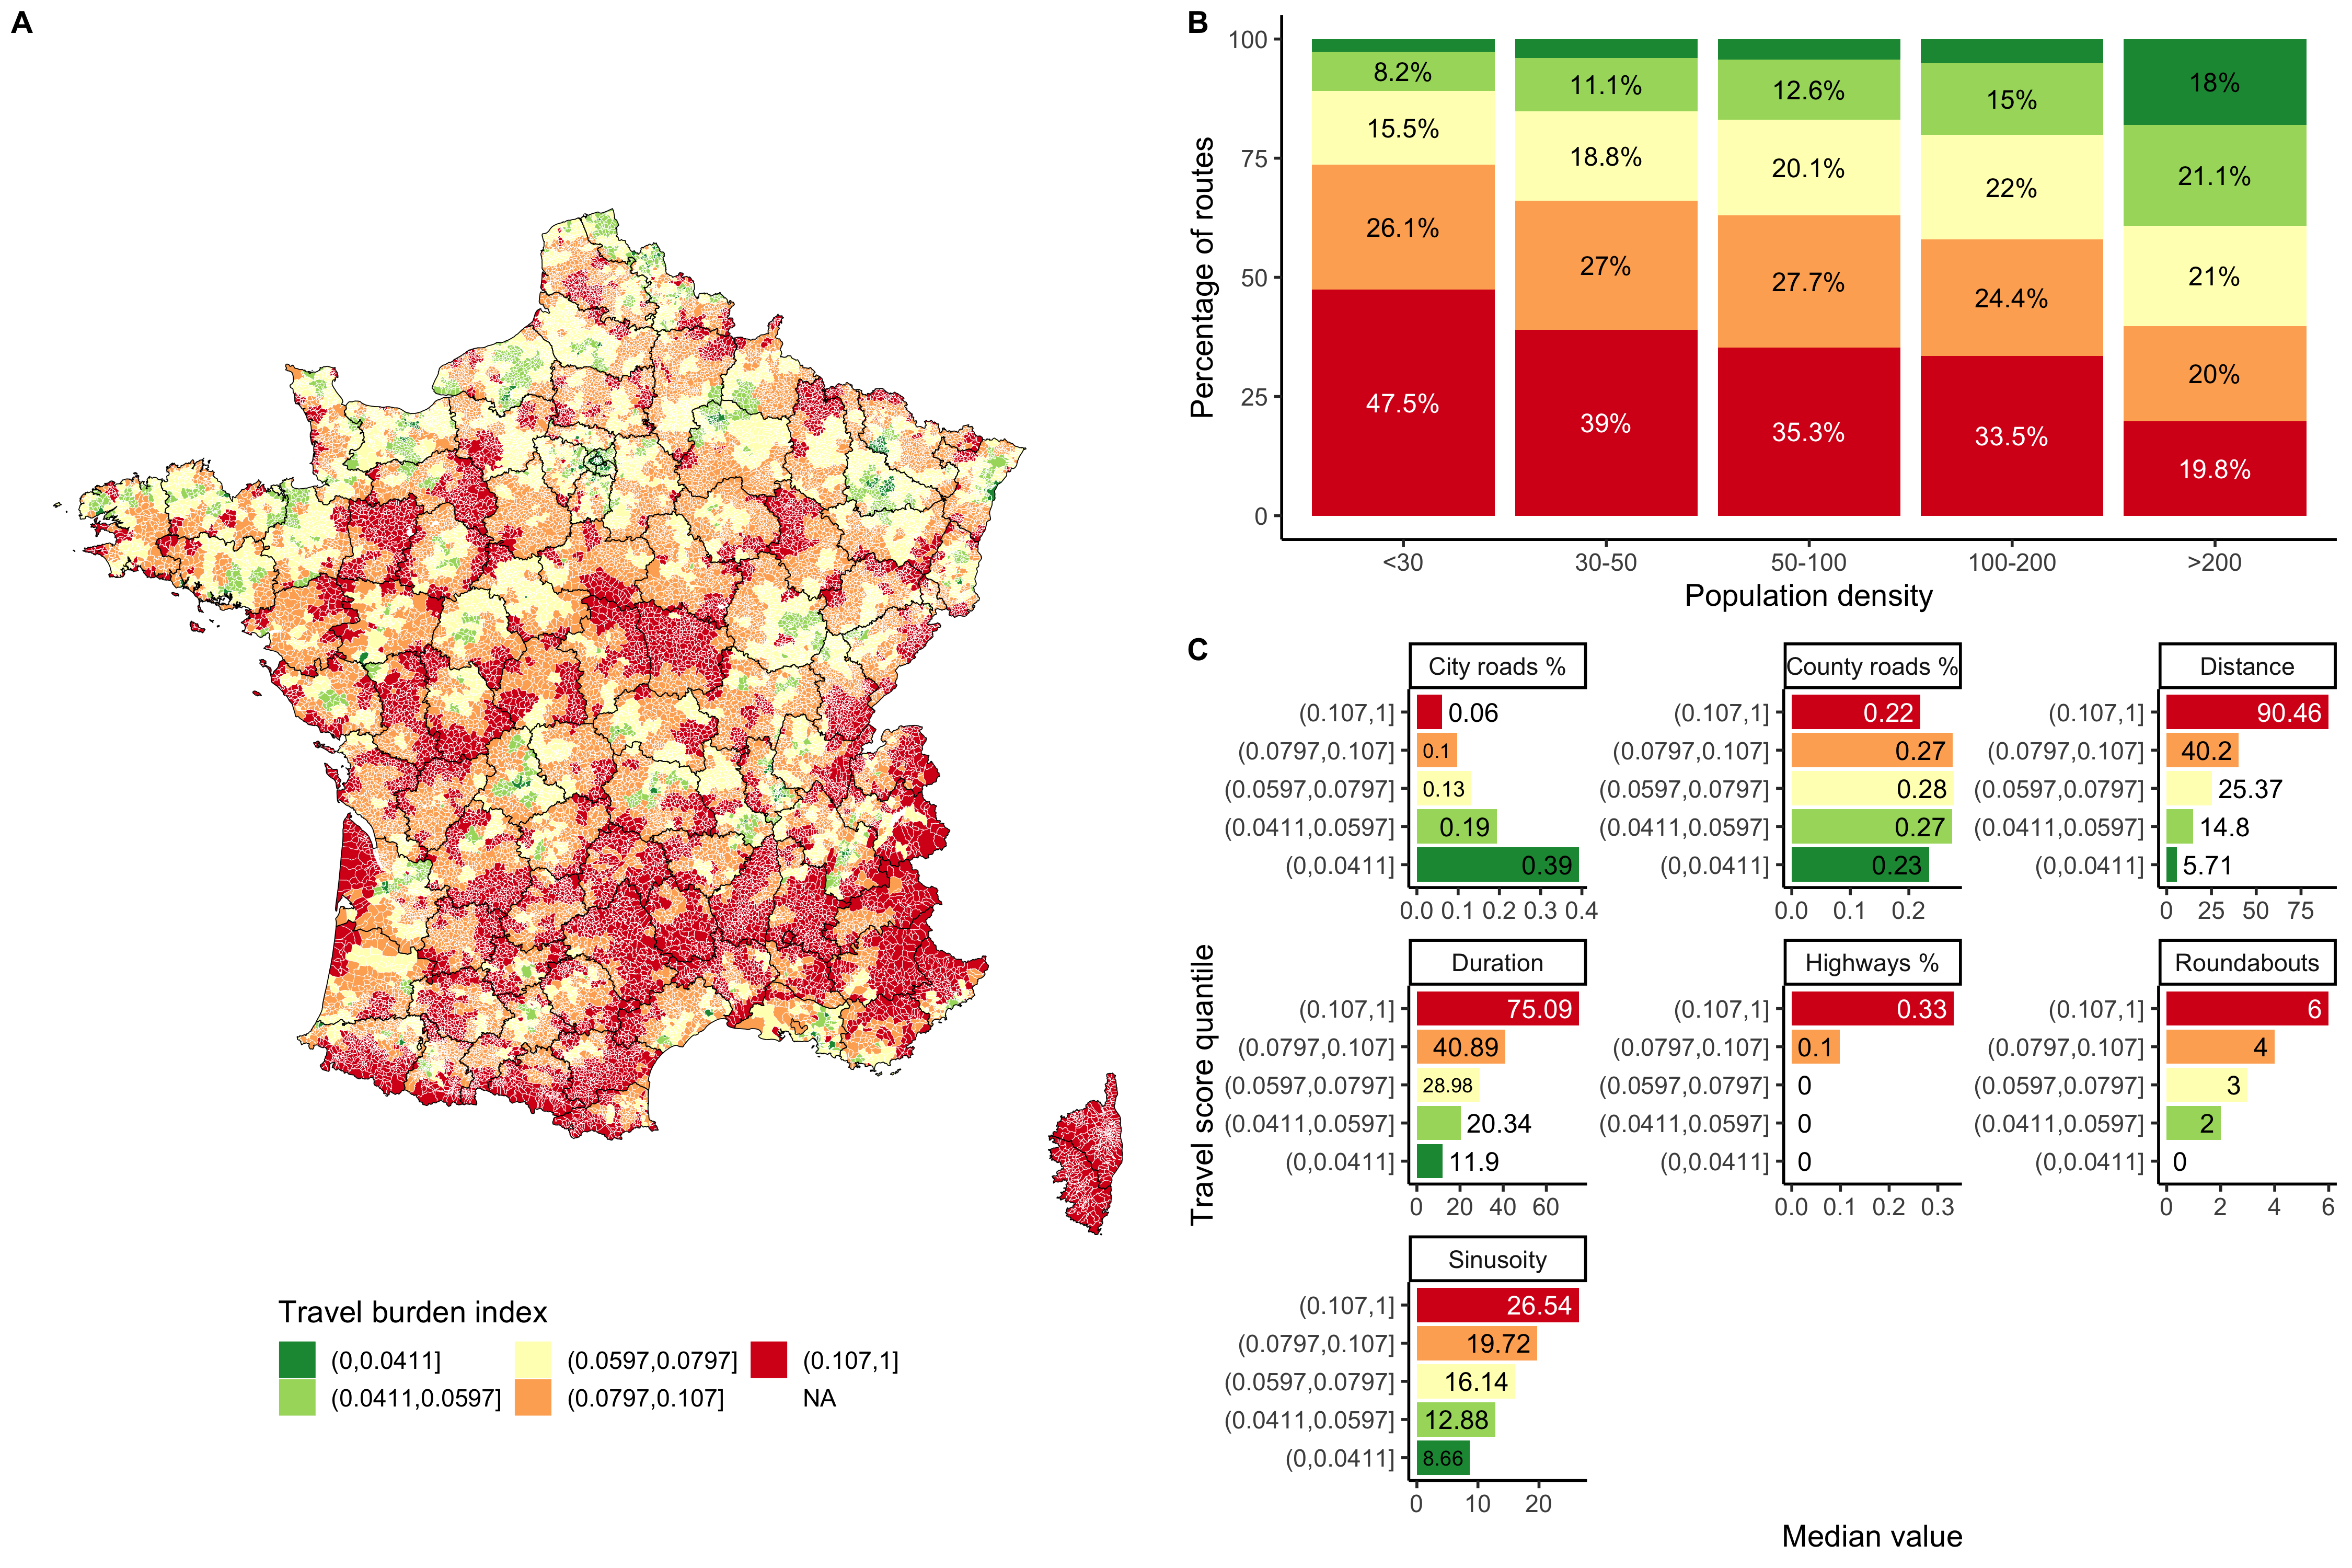
\includegraphics[width=0.9\textwidth]{images/co-occurrences/fig2.png}
    \centering
    \caption{ \textbf{Community detection in France.} Foo }
    \label{fig:co-occ-cluster}
\end{figure}


\section{Conclusion}

In this chapter, our goal was to characterize all the care centers in France
with medicine, surgery or obstetric activity. After gathering health statistics
on these hospitals, we ran clustering algorithm to automatically label each
center in terms of oncology specialization. The clustering algorithm
successfully groups similar hospitals and lets us identify the care centers best
suited for oncology care. Some variables in the \ac{sae} survey are declarative
and potentially differ from the reality. We are aware of this bias, but we do
not expect major differences that could distort our clustering results.
Receiving treatment in a care center with surgery, chemotherapy and radiotherapy
activities is easier for the patient and leads to better care pathways. Care
centers from cluster 1 will be the better choice for cancer treatment and
correspond to modern oncology care specifications. However, these centers are a
minority and sparsely located, essentially in dense areas and in large cities.
While the inhabitants of large cities and metropolitan areas will have no
problem reaching them, rural areas residents live far away from these centers.
This population often has better access to care centers from intermediate
clusters. Such centers do not have all the key services and the patients are
more likely to visit multiple hospitals during their care pathways. Longer
drives to reach a more specialized care center could be considered more
acceptable for surgery, where the hospital volume and surgeon expertise matter.
However, for more frequent interventions like chemotherapy and radiotherapy
especially, patients should prioritize short travels. There is a tradeoff to be
found by patients, between care center proximity and care center expertise. This
dilemma will be more frequent for patients living in rural areas than patients
living in dense cities with large care centers nearby. The different levels of
oncology specialization and the uneven spatial distribution of the oncology
hospitals should be a reason to improve collaborations between hospitals.
If the hospitals with less expertise work closely with oncology dedicated
hospitals, the risks for patients to receive inadequate treatment might be
lowered.
